\documentclass[11pt,a4paper]{article}
\usepackage[T1]{fontenc}
\usepackage[utf8]{inputenc}
\usepackage{lmodern}
\usepackage{amsmath,amssymb,amsthm,mathtools,mathrsfs}
\usepackage{graphicx,float,xcolor,multicol}
\usepackage[shortlabels]{enumitem}
\usepackage[margin=27mm]{geometry}
\usepackage{microtype,needspace,placeins}
\usepackage{tikz,tikz-cd}
\usetikzlibrary{arrows.meta,calc,positioning,patterns,decorations.pathreplacing}
\usepackage[colorlinks=true,linkcolor=teal,urlcolor=teal,citecolor=teal]{hyperref}
\setlength{\parindent}{0pt}
\setlength{\parskip}{.6em}
\setcounter{secnumdepth}{0}
\allowdisplaybreaks
\raggedbottom
\providecommand{\cross}{\times}
\DeclareUnicodeCharacter{2020}{\ensuremath{\dagger}}
\DeclareMathOperator{\supp}{supp}
\DeclareMathOperator*{\esssup}{ess\,sup}
\providecommand{\chapter}{\section}
\newenvironment{tool}[2]{\subsection*{Tool #1 --- #2}}{}
\newcommand{\ToolRef}[1]{Tool #1}
\newcommand{\FigureTag}[2]{\textit{Figure #1}}
\newcommand{\Result}[1]{\subsection*{#1}}
\newcommand{\Application}[1]{\subsubsection*{Application\if\relax\detokenize{#1}\relax\else\space--- #1\fi}}
\newcommand{\ProofHeading}{\par\textit{Proof.}\space}
\newcommand{\ProofOf}[1]{\par\textit{Proof of #1.}\space}
\newcommand{\RemarkHeading}{\par\textbf{Remark.}\space}
\newcommand{\NoteHeading}{\par\textbf{Note.}\space}
\newcommand{\ExerciseHeading}{\par\textbf{Exercise.}\space}

% Rendering support only; mathematical text is in each independent post.
\usepackage{booktabs,array,longtable}
\definecolor{HandoutBlue}{HTML}{2F6690}
\definecolor{HandoutNavy}{HTML}{17365D}
\newtheorem{theorem}{Theorem}
\newtheorem{lemma}[theorem]{Lemma}
\newtheorem{proposition}[theorem]{Proposition}
\newtheorem{corollary}[theorem]{Corollary}
\newtheorem{conjecture}[theorem]{Conjecture}
\newtheorem{definition}{Definition}
\newtheorem{example}{Example}
\newtheorem{namedtoolcounter}{Tool}
\newenvironment{namedtool}[1]{\begin{namedtoolcounter}[#1]}{\end{namedtoolcounter}}
\newtheorem*{claim}{Claim}
\newtheorem*{remark}{Remark}
\newtheorem*{exercise}{Exercise}
\newtheorem*{question}{Question}
\newtheorem*{observation}{Observation}
\newcommand{\SourceChapter}[2]{\section*{#2}}
\newcommand{\Lecture}[2]{\section*{Lecture #1: #2}}
\newcommand{\unclear}[1]{\textit{[unclear: #1]}}
\newcommand{\sourcegap}{\textit{[unfinished in the source]}}
\DeclareMathOperator{\dist}{dist}
\DeclareMathOperator{\id}{id}
\DeclareMathOperator{\Hol}{Hol}
\DeclareMathOperator{\Per}{Per}
\DeclareMathOperator{\Fix}{Fix}
\DeclareMathOperator{\diam}{diam}
\DeclareMathOperator{\Var}{Var}
\DeclareMathOperator{\Leb}{Leb}
\DeclareMathOperator{\Hom}{Hom}
\DeclareMathOperator{\End}{End}
\DeclareMathOperator{\Ann}{Ann}
\DeclareMathOperator{\Spec}{Spec}
\DeclareMathOperator{\Max}{Max}
\DeclareMathOperator{\Ob}{Ob}
\DeclareMathOperator{\Tor}{Tor}
\DeclareMathOperator{\Ass}{Ass}
\DeclareMathOperator{\Mor}{Mor}
\DeclareMathOperator{\Fun}{Fun}
\DeclareMathOperator{\Nat}{Nat}
\DeclareMathOperator{\Cone}{Cone}
\DeclareMathOperator{\MCG}{MCG}
\DeclareMathOperator{\Aut}{Aut}
\DeclareMathOperator{\Deck}{Deck}
\DeclareMathOperator{\SL}{SL}
\DeclareMathOperator{\PSL}{PSL}
\DeclareMathOperator{\Area}{Area}
\DeclareMathOperator{\im}{im}
\DeclareMathOperator{\PSh}{PSh}
\newcommand{\CRing}{\mathsf{CRings}}
\newcommand{\AMod}{A\text{-}\mathsf{Mod}}
\newcommand{\Ab}{\mathsf{Ab}}
\newcommand{\Z}{\mathbb Z}
\newcommand{\Q}{\mathbb Q}
\newcommand{\R}{\mathbb R}
\newcommand{\C}{\mathbb C}
\newcommand{\N}{\mathbb N}
\newcommand{\kk}{\mathbb k}
\renewcommand{\aa}{\mathfrak a}
\newcommand{\bb}{\mathfrak b}
\newcommand{\pp}{\mathfrak p}
\newcommand{\qq}{\mathfrak q}
\newcommand{\mm}{\mathfrak m}
\newcommand{\nn}{\mathfrak n}
\newcommand{\rad}{\mathrm r}
\newcommand{\cat}[1]{\mathsf{#1}}
\setcounter{secnumdepth}{0}
\allowdisplaybreaks

\graphicspath{{figures/complex-dynamics-notes/}}
\begin{document}
\section*{The Mapping Theorem and Invariant Complex Structures}
% BLOG-CONTENT-BEGIN
An ellipse field on a Riemann surface is essentially an ellipse, modulo scaling, chosen in the tangent plane $T_zS$ for almost every $z\in S$. It is the pullback of a circle field via the expression $\mu(z)\,d\overline z/dz$.

The measurable Riemann mapping theorem says that a measurable Beltrami coefficient $\mu$ with $\|\mu\|_\infty<1$ can be integrated by a quasiconformal homeomorphism. On $\widehat{\mathbb C}$, the solution is unique after fixing three points; the plane and disk versions require their corresponding normalizations.

This is also called the integrability theorem or measurable Riemann mapping theorem. We shall see an elementary example in which the mapping theorem joins forces with Weyl's lemma to change the quantitative features of dynamics while keeping its topology the same.
% Source page 2
Start with $M_0\colon\mathbb D\to\mathbb D$, $z\mapsto\lambda_0z$. View this as a map $\mathbb D^*\to\mathbb D^*$ and lift it to the universal cover $\mathbb H_\ell$.
\begin{figure}[H]\centering
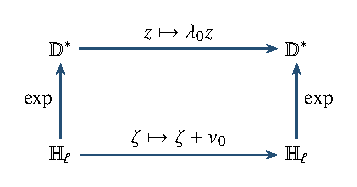
\includegraphics[width=.42\textwidth]{cd6-fig-01.pdf}
\FigureTag{CD6.1}{fig:cd6-01}
\end{figure}
Here $v_0=\log\lambda_0$. Let $L_v$ be the real-linear map on $\mathbb H_\ell$ given by $a\zeta+b\overline\zeta$, where
\[
a=\frac{v+\overline v_0}{v_0+\overline v_0},\qquad
b=\frac{v-v_0}{v_0+\overline v_0}.
\]
The map $L_v$ conjugates $\zeta\mapsto\zeta+v_0$ to $\zeta\mapsto\zeta+v$.
\begin{figure}[H]\centering
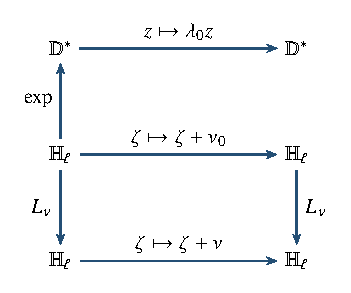
\includegraphics[width=.43\textwidth]{cd6-fig-02.pdf}
\FigureTag{CD6.2}{fig:cd6-02}
\end{figure}
% Source page 3
Finally descend $\zeta\mapsto\zeta+v$ to $\mathbb D^*$, obtaining the following diagram.
\begin{figure}[H]\centering
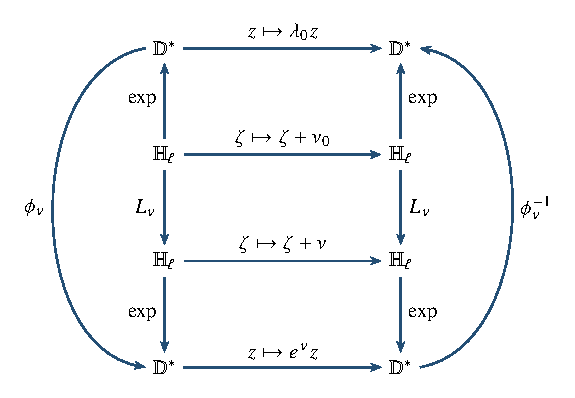
\includegraphics[width=.62\textwidth]{cd6-fig-03.pdf}
\FigureTag{CD6.3}{fig:cd6-03}
\end{figure}
This is an instance in which a holomorphic map is quasiconformally conjugate to another holomorphic map. Here we constructed the conjugacy explicitly. Alternatively, pull back the circle field $\mu_0$ on the bottom copy of $\mathbb D^*$ to obtain $\mu_v=\phi_v^*\mu_0$, then appeal to the mapping theorem. It gives a $K$-quasiconformal map $\phi_v\colon\mathbb D\to\mathbb D$ pulling back the circle field. But how can we ensure that $\phi_v\circ(z\mapsto\lambda_0z)\circ\phi_v^{-1}$ is conformal?
% Source page 4
Usually quasiconformal conjugation does not yield a holomorphic map. It does yield a dynamical conjugate: a map with essentially the same dynamics, but with quantities of our choosing. In the preceding example we changed the multiplier from $\lambda_0$ to $e^v$! In some lucky cases the following is prescribed.
\setcounter{definition}{14}\begin{definition}[$K$-quasiregular map]
A map $g\colon U\to\mathbb C$, $U\subseteq\mathbb C$, is $K$-quasiregular if $g=f\circ\phi$, where $\phi\colon U\to\phi(U)$ is $K$-quasiconformal and $f\colon\phi(U)\to g(U)$ is holomorphic.
\end{definition}
\setcounter{theorem}{24}\begin{lemma}[Surgery lemma]\label{cd6:surgery}
Let $g\colon S\to S$, where $S\cong\mathbb C$ or $\widehat{\mathbb C}$, be quasiregular. If $\mu$ is a $g$-invariant Beltrami form with $\|\mu\|_\infty=k<1$, then there is a quasiconformal map $\phi:S\to X$ such that $f=\phi\circ g\circ\phi^{-1}:X\to X$ is holomorphic, with $X=\mathbb C$ or $\widehat{\mathbb C}$.
\end{lemma}
\begin{proof}
The mapping theorem supplies $\phi\colon S\to X$ in the following diagram; $\mu_0$ denotes the circle field.
\begin{figure}[H]\centering
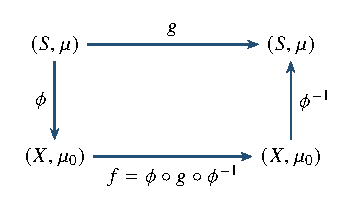
\includegraphics[width=.50\textwidth]{cd6-fig-04.pdf}
\FigureTag{CD6.4}{fig:cd6-04}
\end{figure}
Then $f^*\mu_0=\mu_0$, so $f$ is $1$-quasiregular and therefore holomorphic by Weyl's lemma.
\end{proof}
% Source page 5
Taking our cue from this lemma, after surgically altering the dynamics quantitatively we want to retain a holomorphic map so that complex analysis remains available. For that, the conjugate $\phi\circ g\circ\phi^{-1}$ must be a Beltrami-form-preserving quasiregular map.

In our original example, $\phi_v\circ(z\mapsto\lambda_0z)\circ\phi_v^{-1}$ was conformal, hence circle-field-preserving and $1$-quasiregular. To stitch the incision after changing the quantitative dynamics, we must hope for an ellipse-field-preserving quasiregular map. Otherwise it is surgery gone wrong! More perspective on quasiregular maps may shed light on this.
\setcounter{definition}{15}\begin{definition}[Second definition of $K$-quasiregularity]
A map $g\colon U\to\mathbb C$ is $K$-quasiregular if it is locally $K$-quasiconformal except on a discrete set.
\end{definition}
\setcounter{definition}{16}\begin{definition}[Third definition of $K$-quasiregularity]
For every $z\in U$, there are neighbourhoods $N_z,N_{g(z)}$ of $z,g(z)$, a $K$-quasiconformal map $\psi\colon N_z\to\mathbb D$, and a conformal map $\varphi\colon N_{g(z)}\to\mathbb D$ such that
\[
\varphi\circ g\circ\psi^{-1}(z)=z^d\qquad\text{for some }d\ge1.
\]
\end{definition}
% Source page 6
We show that the three definitions are equivalent; this reveals enough content to perform a good surgery. The implication $(1)\Rightarrow(2)$ is clear.

For $(2)\Rightarrow(1)$, the Lindel\"of property gives a countable family $\{U_i\}_{i\in\mathbb N}$ on each of which $g$ is $K$-quasiconformal except at a discrete set. Then $\partial_zg,\partial_{\overline z}g\in L^2_{\mathrm{loc}}$. Define $\widehat\mu(z)=0$ outside $U_i$, and $\mu(z)=\partial_{\overline z}g(z)/\partial_zg(z)$ inside. There is a map $\widehat\phi\colon\mathbb C\to\mathbb C$ pulling back the circle field to this ellipse field. Put $\phi=\widehat\phi|_{U_i}$ and $f=g\circ\phi^{-1}$.
\begin{figure}[H]\centering
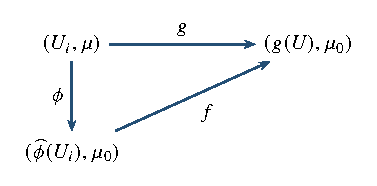
\includegraphics[width=.51\textwidth]{cd6-fig-05.pdf}
\FigureTag{CD6.5}{fig:cd6-05}
\end{figure}
By Weyl's lemma, $f$ is conformal except on a discrete set; continuity makes the singularities there removable.

For $(3)\Rightarrow(1)$, if $\varphi\circ g\circ\psi^{-1}=z^d$ and $d=1$, we are done. If $d>1$, the map is a local homeomorphism except at discrete points, because $0$ is the only point where this fails.
% Source page 7
Those points are isolated, so $(3)\Rightarrow(2)\Rightarrow(1)$.

For $(1)\Rightarrow(3)$, suppose $g=f\circ\phi$. If $\phi(z)\notin\operatorname{Crit}(f)$, there are neighbourhoods $N_{\phi(z)},N_{g(z)}$ such that $f\colon N_{\phi(z)}\to N_{g(z)}$ is conformally invertible, and $f^{-1}\circ g\circ\phi^{-1}=z^1$.

If $\phi(z)\in\operatorname{Crit}(f)$, choose these neighbourhoods so that $f$ is a branched covering of degree $d$, branched only at $\phi(z)$.
\begin{figure}[H]\centering
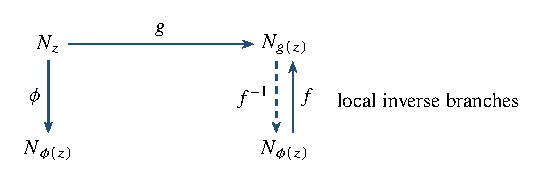
\includegraphics[width=.74\textwidth]{cd6-fig-06.pdf}
\FigureTag{CD6.6}{fig:cd6-06}
\end{figure}
Now consider the following self-explanatory diagram. Shrink $N_{g(z)}$ to be simply connected, take its Riemann map $R$, and lift $R$ to $\widetilde R$ (basically a deck transformation).
\begin{figure}[H]\centering
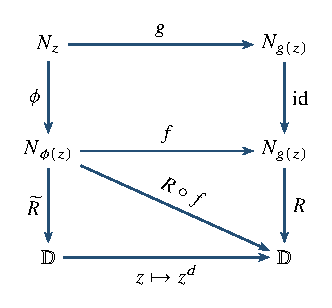
\includegraphics[width=.54\textwidth]{cd6-fig-07.pdf}
\FigureTag{CD6.7}{fig:cd6-07}
\end{figure}
Then $R\circ g\circ(\widetilde R\circ\phi)^{-1}$ is the required map.
% Source page 8
Among the many things one must look out for in a good surgery, knowing one's way around quasiregularity is important. There are deeper principles and schemes, due to Shishikura, governing how and when surgery can be performed. We will see them later. This post is a peek into the role of quasiconformality in loosening dynamics. As promised, the flexibility in conformality is deeply connected with flexibility in the resulting dynamics.
\subsection{Addendum: two properties of quasiconformal maps}
\begin{enumerate}
\setcounter{enumi}{0}\item Local H\"older estimate: if $\varphi:U\to V$ is $K$-quasiconformal and $E\Subset U$, then there is $C_E>0$ such that
\[
|\varphi(z_1)-\varphi(z_2)|\le C_E|z_1-z_2|^{1/K}\qquad(z_1,z_2\in E).
\]
\setcounter{enumi}{1}\item The family of $K$-quasiconformal homeomorphisms $\varphi\colon\widehat{\mathbb C}\to\widehat{\mathbb C}$ fixing $0,1,$ and $\infty$ is closed in the $C^0$ topology, and in fact compact. For a sequence $\{\varphi_n\}_{n\in\mathbb N}$, equicontinuity on the compact sphere gives sequential compactness by Arzel\`a--Ascoli. Applying the same argument to $\varphi_n^{-1}$ shows that the limit $\varphi$ is a homeomorphism. Its $K$-quasiconformality follows from the geometric definition.
\end{enumerate}
% Source page 9
\subsection{Addendum: full proof of Weyl's lemma}
Let $f:D\to\mathbb C$ be continuous and suppose $f_{\bar z}=0$ in the sense of distributions. Fix a compact set $K\subset D$, choose $U_K$ with $K\subset U_K\subset\overline{U_K}\subset D$, and let $\eta\in C_0^\infty(D)$ be identically one on $U_K$.

Set
\[
\varphi(z)=\begin{cases}
C\exp\!\left(-\dfrac1{1-|z|^2}\right),&z\in\mathbb D,\\
0,&\text{otherwise},
\end{cases}
\qquad\iint_{\mathbb D}\varphi(z)\,dx\,dy=1,
\]
choosing $C$ accordingly. Define $\varphi_n(z)=n^2\varphi(nz)$ and
\[
f_n(w)=\varphi_n*(\eta f)(w)
=\iint_{\mathbb C}\varphi_n(w-z)\eta(z)f(z)\,dx\,dy.
\]
For $w\in K$ and all sufficiently large $n$, the support of $z\mapsto\varphi_n(w-z)$ lies where $\eta=1$. Hence $(f_n)_{\bar z}(w)=\varphi_n*(\eta f)_{\bar z}(w)=0$, so $f_n$ is holomorphic on a neighbourhood of $K$.

For large $n$, $\operatorname{supp}(\varphi_n)=\overline{\mathbb D}_{1/n}$. Compactness of $K$ gives $n$ such that $B(w,1/n)\subset U_K$ for every $w\in K$.
% Source page 10
Since $\eta=1$ on $U_K$,
\begin{align*}
f_n(w)&=\iint_{|w-z|<1/n}\varphi_n(w-z)f(z)\,dx\,dy\\
&=\int_0^{2\pi}\int_0^{1/n}
\frac{Cn^2f(w+re^{i\theta})r}{\exp(1/(1-n^2r^2))}\,dr\,d\theta,
\end{align*}
while $f(w)=\iint_{\mathbb D}f(w)\varphi(z)\,dx\,dy$. Thus $|f_n-f|\to0$ uniformly on $K$ by uniform continuity of $f$ on a compact neighbourhood of $K$. Hence $f_n\to f$ uniformly on compact sets and $f$ is holomorphic.
\begin{remark}
This immediately implies the Looman--Menchoff theorem.
\end{remark}
% BLOG-CONTENT-END
\end{document}
